\documentclass{article}
\usepackage{amsmath}
\usepackage[mathletters]{ucs}
\usepackage[utf8x]{inputenc}
\usepackage[margin=1.5in]{geometry}
\usepackage{enumerate}
\newtheorem{theorem}{Theorem}
\usepackage[dvipsnames]{xcolor}
\usepackage{pgfplots}
\setlength{\parindent}{0cm}
\usepackage{graphics}
\usepackage{graphicx} % Required for including images
\usepackage{subcaption}
\usepackage{subcaption}
\usepackage{bigintcalc}
\usepackage{pythonhighlight} %for pythonkode \begin{python}   \end{python}
\usepackage{appendix}
\usepackage{arydshln}
\usepackage{physics}
\usepackage{tikz-cd}
\usepackage{booktabs} 
\usepackage{adjustbox}
\usepackage{mdframed}
\usepackage{relsize}
\usepackage{physics}
\usepackage{cancel}
\usepackage[thinc]{esdiff}
\usepackage{fixltx2e}
\usepackage{esint}  %for lukket-linje-integral
\usepackage{xfrac} %for sfrac
\usepackage{hyperref} %for linker, må ha med hypersetup
\usepackage[noabbrev, nameinlink]{cleveref} % to be loaded after hyperref
\usepackage{amssymb} %\mathbb{R} for reelle tall, \mathcal{B} for "matte"-font
\usepackage{listings} %for kode/lstlisting
\usepackage{verbatim}
\usepackage{graphicx,wrapfig,lipsum,caption} %for wrapping av bilder
\usepackage{mathtools} %for \abs{x}
\usepackage[norsk]{babel}
\definecolor{codegreen}{rgb}{0,0.6,0}
\definecolor{codegray}{rgb}{0.5,0.5,0.5}
\definecolor{codepurple}{rgb}{0.58,0,0.82}
\definecolor{backcolour}{rgb}{0.95,0.95,0.92}
\pagecolor[rgb]{0.075,0.075,0.075} \color[rgb]{1,1,1} %TODO: Slett når ferdig%
\lstdefinestyle{mystyle}{
    backgroundcolor=\color{backcolour},   
    commentstyle=\color{codegreen},
    keywordstyle=\color{magenta},
    numberstyle=\tiny\color{codegray},
    stringstyle=\color{codepurple},
    basicstyle=\ttfamily\footnotesize,
    breakatwhitespace=false,         
    breaklines=true,                 
    captionpos=b,                    
    keepspaces=true,                 
    numbers=left,                    
    numbersep=5pt,                  
    showspaces=false,                
    showstringspaces=false,
    showtabs=false,                  
    tabsize=2
}

\lstset{style=mystyle}
\author{Oskar Idland}
\title{FYS2140 - Oblig 1}
\date{}
\begin{document}
\maketitle
\newpage
\part*{\underline{A Diskusjonsoppgaver}}
\section*{Oppgave 1 Kontinuitet og Kvantisering}
\subsection*{a) Størrelser i klassisk fysikk}
\subsubsection*{\textbf{Bevegelsesmengde $p$:}}
Bevegelsesmengde er en kontinuerlig størrelse ettersom hastighet er en kontinuerlig størrelse. 

\subsubsection*{\textbf{Elektrisk ladning $q$:}}
Elektrisk ladning er en diskré størrelse ettersom det er definert ut fra ladningen til et enkelt elektron. 

\subsubsection*{\textbf{Energi $E$}}
Energi er en kontinuerlig størrelse. 

\subsection*{b) Størrelser i kvantefysikk}  
\subsubsection*{\textbf{Bevegelsesmengde $p$:}}
Bevegelsesmengde er en diskré størrelse ettersom energien til partikler er diskret.

\subsubsection*{\textbf{Elektrisk ladning $q$:}}
Elektrisk ladning er en diskré størrelse ettersom det er definert ut fra ladningen til et enkelt elektron. 

\subsubsection*{\textbf{Energi $E$}}
Energi er en diskré størrelse 
  

\begin{figure}
\subsection*{c)}
    \centering
    \begin{subfigure}{.45\textwidth}
      \centering
      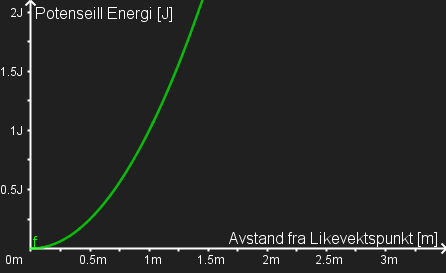
\includegraphics[width = \textwidth]{Figures/A.1.c.i.png}
      \caption{Potensiell energi i en gjør som funksjon av avstanden $x$ fra likevektspunktet}
      \label{subfig: A.1.c.i}
    \end{subfigure}
    \hfill
    \begin{subfigure}{.45\textwidth}
      \centering
      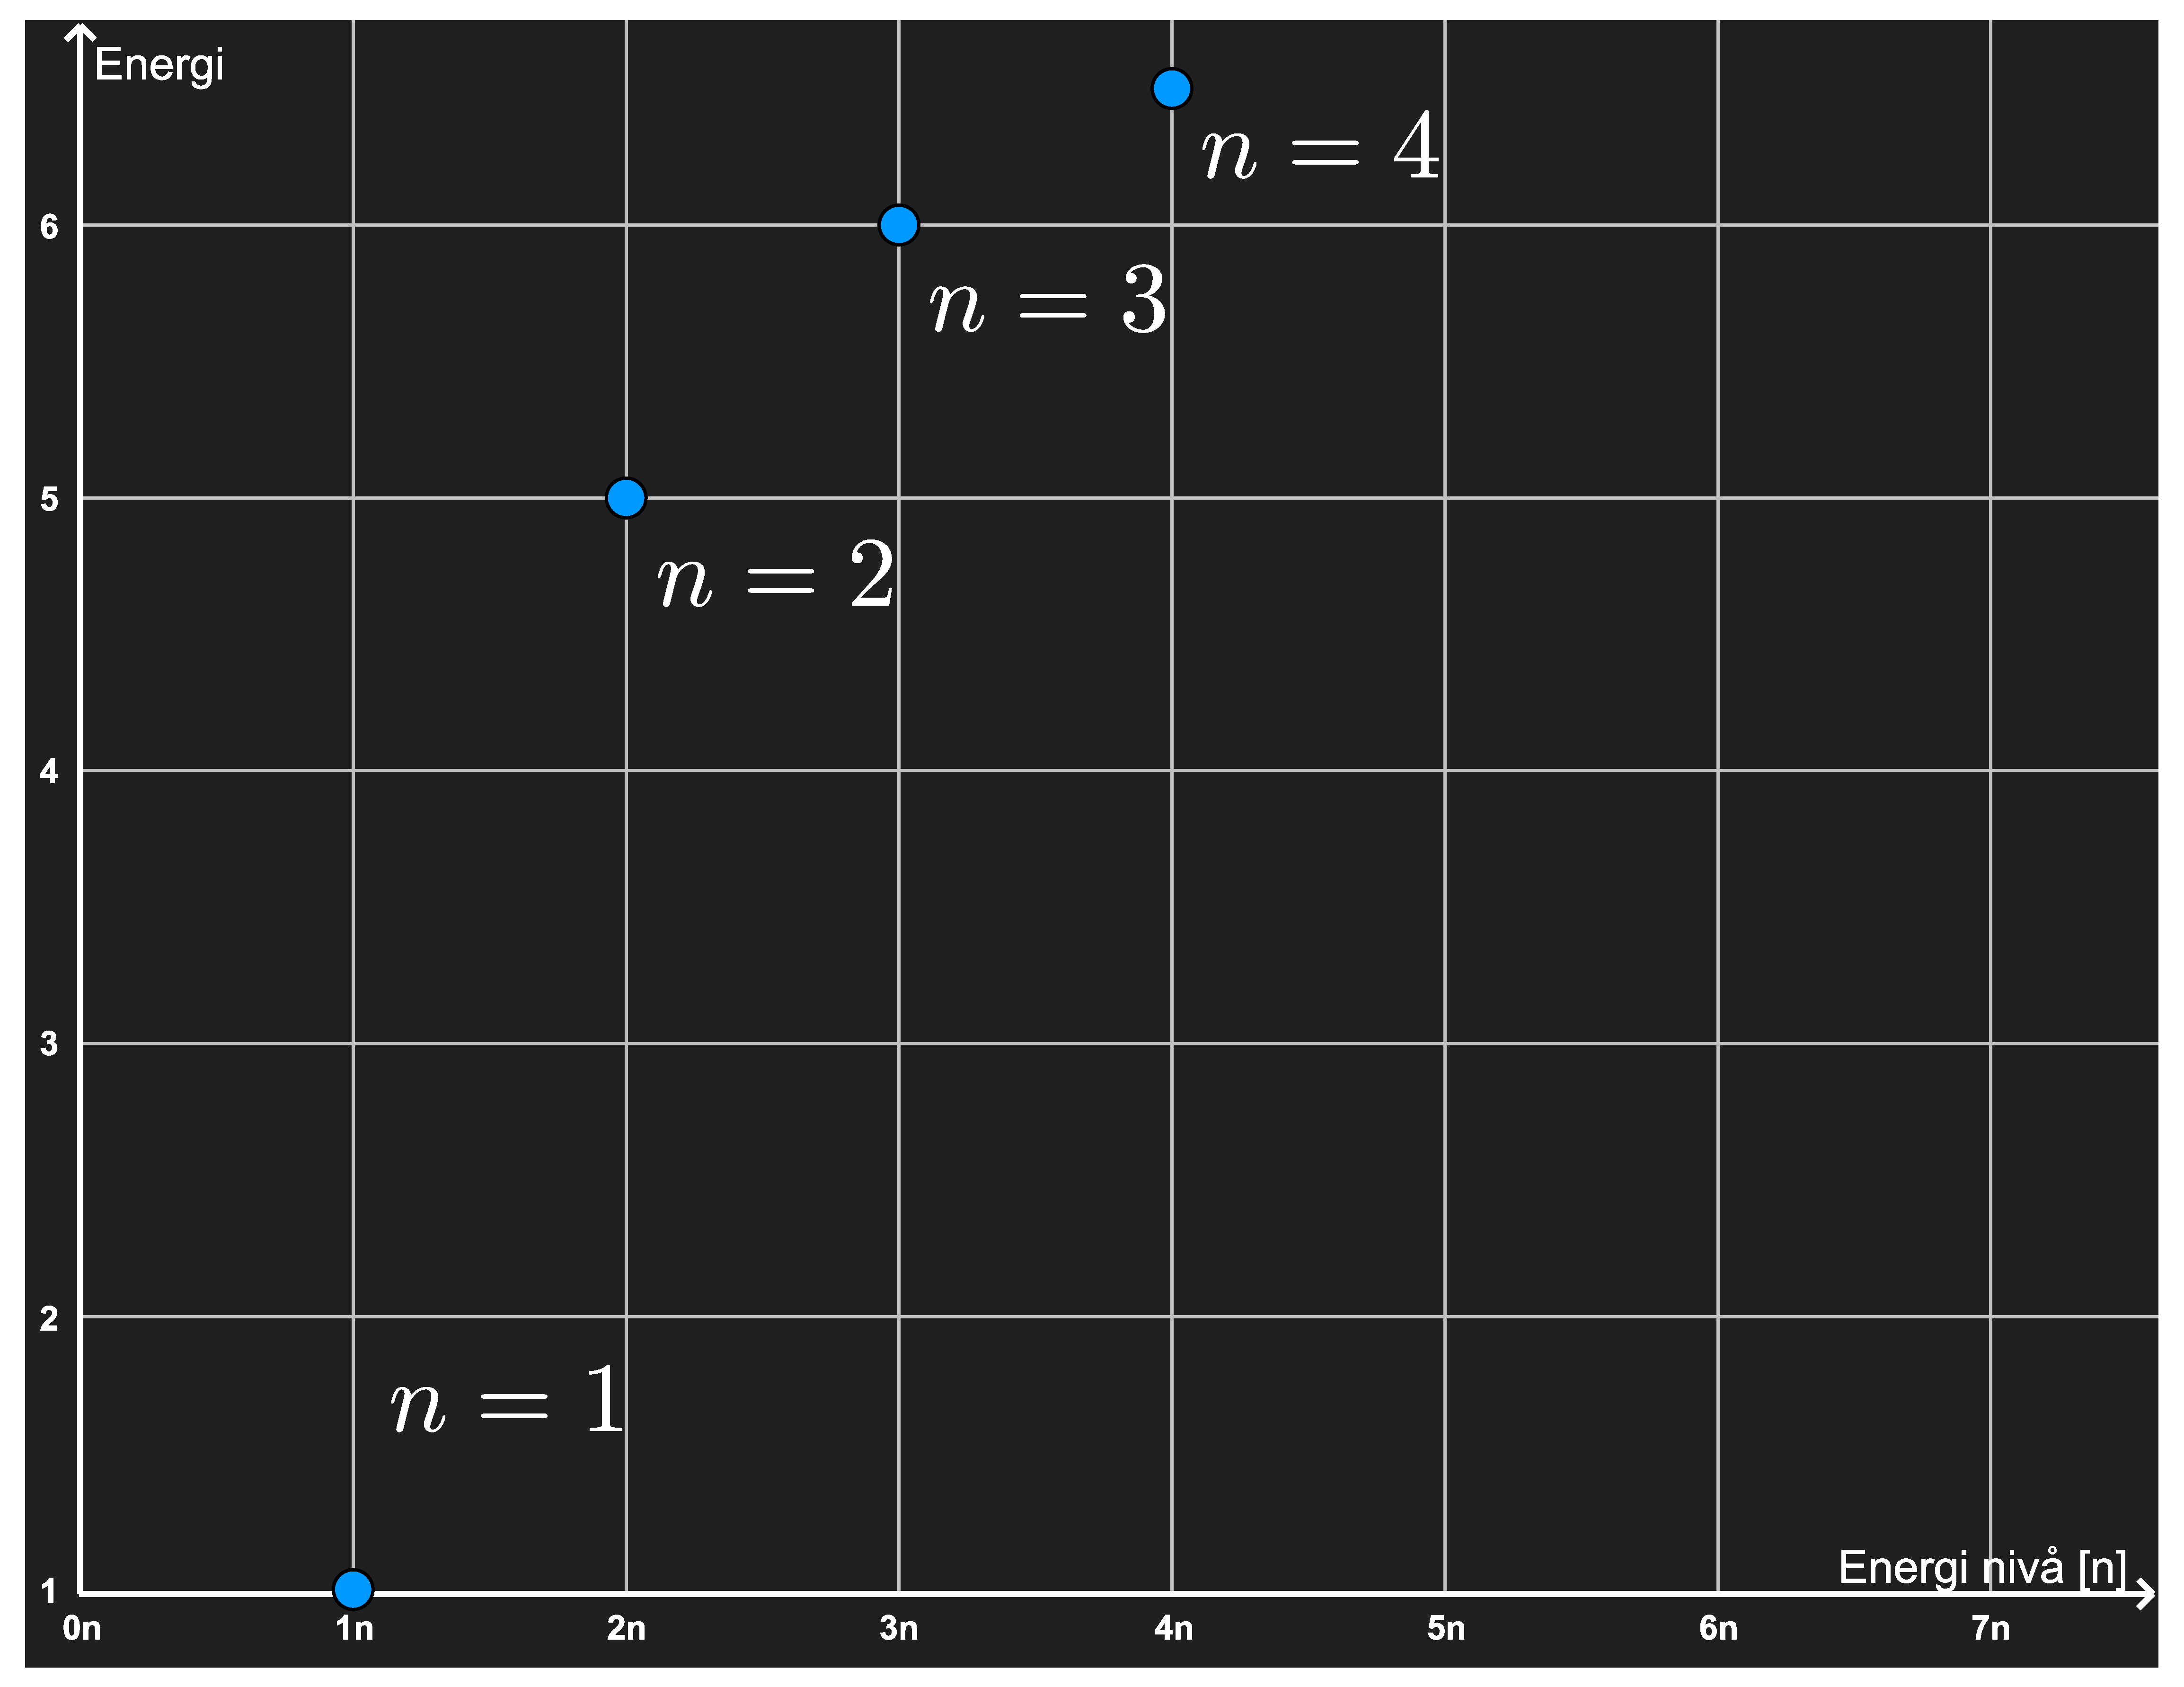
\includegraphics[width = \textwidth]{Figures/A.1.c.ii.pdf}
      \caption{Energien til et elektron i et hydrogenatom som en funksjon av energinivå $n$}
      \label{subfig: A.1.c.ii}
    \end{subfigure}
    \hfill
    \caption{Grafer som viser forskjellen på kontinuerlige og diskrete størrelser}
    \label{fig: A.1.c}
\end{figure}



\newpage
\section*{Oppgave 2 Determinisme og Statistisk Fordeling}
\subsection*{a)}
For å vite hvor en ball havner etter den har blitt kastet må vi vite dens startposisjon $r_0$ og dens hastighetsvektor $\vec{v}$. Usikkerheter kan komme fra vår evne til å måle både hastighet og startposisjon. I klassisk fysikk er dette kontinuerlige verdier som vil være umulig å få helt nøyaktig. 

\subsection*{b)}
For å vite akkurat hvor den ville havnet måtte vi hatt den eksakte startposisjon $r_0$ og dets hastighetsvektor $\vec{v}$. I kvantefysikken er det umulig å vite begge to samtidig og dermed umulig å vite nøyaktig hvor den havner. Det eneste vi kan vite er sannsynligheten for hvor partikkelen kan befinne seg og hvilke hastigheter den kan ha. Dette kan gi oss da en sannsynlighet for hvor den kommer til å havne. 

\begin{figure}
\subsection*{c)}
    \centering
    \begin{subfigure}{.49\textwidth}
      \centering
      
\includegraphics[width = \textwidth]{Figures/A.2.b.1.png}
      \caption{100 baller som kastet likt etter hverandre mot en vegg}
      \label{fig: 100 baller}
    \end{subfigure}
    \hfill
    \begin{subfigure}{.49\textwidth}
      \centering
      
\includegraphics[width = \textwidth]{Figures/A.2.b.2.png}
      \caption{100 elektroner som skytes likt etter hverandre mot en vegg}
      \label{fig: 100 elektroner}
    \end{subfigure}
    \hfill
    \caption{Forskjellen på baller og elektroner som oppfører seg klassisk og kvantemekanisk}
    \label{fig: A.2.b}
\end{figure}

\newpage
\part*{\underline{B Regneoppgaver}}
\section*{Oppgave 3 Lek med Komplekse Tall}
\subsection*{a)}
\begin{enumerate}[(i)]
    \item $z = i$
    \[
    z^{*} = - i 
    \]
    \[
    \left| z \right|  = \sqrt{0^2 + 1^2} = 1 
    \]
    \[
    \left| z \right| ^{2} = 1^{2} = 1
    \] 
    \[
    zz^{*}  = -ii = 1 = \left| z \right|^{2}
    \]
    \item $z = 3 + 4i$ 
    \[
    z^{*} = 3 - 4i 
    \] 
    \[
    \left| z \right| = \sqrt{3^2 + 4^2} = 5 
    \]
    \[
    \left| z \right| ^{2} = 5^{2} = 25
    \] 
    \[
    zz^{*} = \left( 3 + 4i  \right) \left( 3 - 4i \right) = 9 - \cancel{12i} + \cancel{12i} - 16ii = 25 = \left| z \right| ^{2}
    \]
    \item $z = -3$
    \[
    z^{*} = -3
    \]
    \[
    \left| z \right| = \sqrt{\left( -3 \right) ^{2}} = 3
    \]
    \[
    \left| z \right| ^{2} = 3^{2} = 9
    \]
    \[
    zz^{*} = -3 ⋅ -3 = 9 = \left| z \right| ^{2}
    \]
    \item $z = 1 + i$
    \[
    z^{*} = 1 - i 
    \]
    \[
    \left| z \right| = \sqrt{1^2 + (-1)^2} = \sqrt{2}
    \]
    \[
    \left| z \right| ^{2} = \sqrt{2}^{2} = 2
    \]
    \[
    zz^{*} = \left( 1 + i \right) \left( 1 - i \right) = 1 - \cancel{i} + \cancel{i} - i^{2} = 1 + 1 = 2 = \left| z \right| ^{2}
    \]
\end{enumerate}

\subsection*{b)}
I følgende oppgaver vil vi bruke relasjonen $z_1 / z_2 = z_1 z_2 ^{*} \left| z_2 \right| ^{2}$
\begin{enumerate}[(i)]
    \item $\frac{3 + 4i}{1 - 2i}$
    \[
    z_2^{*} = 1 + 2i, \quad \left| z_2 \right| ^{2} = \sqrt{1^2 + (-2)^2}^{2} = 5
    \]
    \[
    \left( 3 + 4i \right) \left( 1 + 2i  \right) / 5 = \frac{3 + 6i + 4i - 8}{5} = -1 + 2 i
    \]
    \item $\frac{\sqrt{3} + i}{(1 - i)(\sqrt{3}-i)}$
    Vi ønsker å bli kvitt røttene og multipliserer med $\sqrt{3} - i$ oppe og nede. 
    \[
    \frac{\sqrt{3} + i}{(1 - i)(\sqrt{3}-i)} \frac{\sqrt{3}- i}{\sqrt{3}-i} = \frac{4}{(1-i) ⋅ 2} = \frac{2}{1 - i}
    \]
    \[
    z_2^{*} = 1 + i,  \quad \left| z_2 \right| ^{2} = \sqrt{1^2 + (-1)^2}^{2} = 2
    \]
    \[
    \frac{2 ⋅ \left( 1 + i \right)}{2} = 1 + i
    \]
\end{enumerate}
 
\subsection*{c)}
I følgende oppgaver bruker vi at $e^{i θ} = \cos θ + i \sin θ$, hvor $θ ∈ [-π, π]$. 
\begin{enumerate}[(i)]
    \item $z = 2i$
    \[
    z = 2 e^{i \frac{π}{2}}
    \] 
    \item $z = -6 + 6 \sqrt{3}i$.
    \[
    r = \sqrt{6^2 + 6^2 \sqrt{3}^2} = 12 \quad , \quad θ = \arctan \left( \frac{6 \sqrt{3}}{-6} \right) = \frac{2}{3} π
    \]
    \[
    z = 12 e^{i \frac{2}{3} π}
    \]  
    \item $z = -1$
    \[
    z = 1 e^{i π}
    \]
\end{enumerate}
 
\subsection*{d)}
\begin{enumerate}[(i)]
    \item $z_1 = 2e ^{-iπ}$ og $z_2 = 3 e ^{i \frac{π}{3}}$
    \[
    z_1 z_2 = 2 ⋅ 3 e^{i\left( -π + \frac{π}{3} \right) } = 6 e^{-i\frac{2}{3} π}
    \] 
    \item $z_1 = e^{-i \frac{1}{5}π}$ og $z_2 = e^{i \frac{1}{5}π}$
    \[
    z_1 z_2 = 1 ⋅ 1 e^{i \left(\cancel{-\frac{1}{5}π} \cancel{+ \frac{1}{5}π} \right) } = 1
    \]
\end{enumerate}
Ettersom $e^{i \frac{π}{2}} = i$ er å multiplisere med dette det samme som å multiplisere med $i$ som er det samme som å rotere ett komplekst tall med $90^{\circ}$ i positiv retning.

\section*{Oppgave 4 Derivasjon og et par Viktige Diff. ligninger}
\subsection*{a)}
\begin{enumerate}[(i)]
    \item $f(x) = A e^{-ax}$
    \[
    f'(x) = -aA e^{-ax} \quad , \quad f''(x) = a^2 A e^{-ax}
    \] 
    \item $f(x) = A e^{iax}$ 
    \[
    f'(x) = iaA e^{iax} \quad , \quad f''(x) = -a^2 A e^{iax}
    \] 
    \item $f(x) = \sin (ax)$
    \[
    f'(x) = a \cos (ax) \quad , \quad f''(x) = -a^2 \sin (ax)
    \]
\end{enumerate}

\subsection*{b)}
Vi betrakter differensiallikningen 
\[
\frac{\mathrm{d}f(x)}{\mathrm{d}x} = b f(x), \qquad f(0) = 1 \quad , \quad f'(0) = 3
\]
Vi skriver dette på den generelle formen 
\[
r - b = 0
\]
som har løsning $r = b$. Vi kan derfor skrive om løsningen til følgende: 
\[
f(x) = Ce^{bx}. 
\]
Deretter setter vi inn initial betingelsene. 
\[
f(0) = C = 1 ⇒ C = 1
\]
\[
f'(0) = 1 ⋅ b = 3 ⇒ b = 3
\]
Da har vi løsningen
\[
f(x) = e^{3x}
\]
\subsection*{c)}
Vi betrakter differensiallikningen 
\[
\frac{\mathrm{d}^{2}f(x)}{\mathrm{d}x^{2}} = ε f(x) .
\]
Vi skriver dette på den generelle formen
\[
r^{2} - ε = 0
\]
som har løsningene $r = ±  \sqrt{ε}$. Vi kan derfor skrive om løsningen til følgende:
\[
f(x) = A e^{\sqrt{ε}x} + B e^{-\sqrt{ε}x}.
\]
Hvis vi krever at $\lim_{x \to ∞} f(x) = 0$ må $A = 0$ ettersom $\lim_{x \to ∞}e ^{\sqrt{ε}x} = ∞$. \\ 

Hvis vi krever at $\lim_{x \to -∞}f(x) = 0$ må $B = 0$ ettersom $\lim_{x \to -∞}e ^{-\sqrt{ε}x} = ∞$. \\

\begin{figure}[h!]
  \centering
  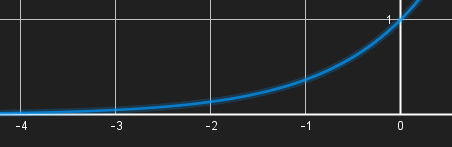
\includegraphics[scale = .75]{Figures/B.4.d.png}
  \caption{$f(x)$ med $B = 0$ og $A = 1$}
  \label{fig: B.4.d}
\end{figure}

\subsection*{d)}
Hvis $ε < 0$ så vil løsningen på ligningen bli kompleks. Da blir løsningen $r = ± i \sqrt{ε}$ som gir oss en funksjon $f(x)$    
\[
 f(x) = A e^{i \left|\sqrt{ε}\right| x} + B e^{-i \left|\sqrt{ε}\right| x} = A( \cos (\left|\sqrt{ε}\right| x) + i \sin (\left|\sqrt{ε}\right| x) ) + B( \cos (\left|\sqrt{ε}\right| x) - i \sin (\left|\sqrt{ε}\right| x) )
\]
\[
f(x) =  A \cos (\left|\sqrt{ε}\right| x) + B \cos (\left|\sqrt{ε}\right| x) + i\left( A \sin (\left|\sqrt{ε}\right| x) - B \sin (\left|\sqrt{ε}\right| x) \right)
\]
\[
f(x) = \left( A + B \right) \cos (\left|\sqrt{ε}\right| x) + i \left( A - B \right) \sin (\left|\sqrt{ε}\right| x)
\]

\section*{Oppgave 5 Litt integralregning}
\subsection*{a)}
\begin{enumerate}[(i)]
    \item 
    \[
    ∫_{-∞}^{∞} e^{-x^{2} - 4x - 1} \ \mathrm{d}x = ∫_{-∞}^{∞} e^{-\left( x^{2} + 2 ⋅ 2x + 1 \right) } \ \mathrm{d}x
    \]
    Bruker Rottmann (2019 s, 155 (51))
    \[
    ∫_{-∞}^{∞} e^{-\left( ax^{2} + 2bx + c \right) } \ \mathrm{d}x = \sqrt{\frac{π}{a}} e^{\frac{b^{2} - ac}{a}}
    \]
    \[
    π e^{\frac{2^{2} - 1}{1}} = π e^{3}  x^2  
    \] 
    \item   
    \[
    ∫_{0}^{∞} xe ^{-2x^{2}} \ \mathrm{d}x
    \]
    Bruker Rottmann (2019 s, 155 (50)) 
    \[
    ∫_{0}^{∞} x^{k} e^{- λx^{2}} \ \mathrm{d}x = \frac{1}{2} λ ^{-\frac{k + 1}{2}} Γ \left( \frac{k + 1}{2}\right) 
    \]
    \[
    \frac{1}{2}2^{- \frac{1 + 1}{2}} Γ\left( \frac{1+1}{2} \right) = \frac{1}{2} 2^{-1} Γ(1)  
    \]
    \[
    \frac{1}{4} 1 = \frac{1}{4}
    \]
\end{enumerate}
\subsection*{b)}
\[
∫_{-∞}^{∞} ∫_{-∞}^{∞} ∫_{-∞}^{∞} e^{-2 \sqrt{x^2 + y^2 + z^2 }} \ \mathrm{d}x \ \mathrm{d}y \ \mathrm{d}z
\]
Vi konverterer til sfæriske koordinater. 
\[
∫_{0}^{∞} ∫_{0}^{2π} ∫_{0}^{π} ρ \sin (θ) e^{-2ρ}  \ \mathrm{d}θ \ \mathrm{d}ϕ \ \mathrm{d}ρ
\]
\[
∫_{0}^{∞} ∫_{0}^{π} 2π ρ \sin (θ) e^{-2ρ} \ \mathrm{d}θ \ \mathrm{d}ρ = ∫_{0}^{∞} 4 ρ e^{-2ρ} \ \mathrm{d}ρ
\]
Vi bruker at 
\[
∫_{0}^{∞} x^{n} e ^{-α x} \ \mathrm{d}x = \frac{1}{α^{n+1}}n!
\]
\[
4π\frac{1}{2^{2}} 1! = π 
\]

\[
\sqrt{\left( x - 1 \right)^{2} } \left(\frac{x}{2}\right) = \sqrt{\left( x - 1 \right)^{2} } 
\left( λ - 2 \right)^2 
\]

\end{document}